
\usepackage{fancyhdr}
\usepackage{lastpage}
\usepackage[utf8]{inputenc}

% Minted for syntax highliting
\usepackage{minted}
\usemintedstyle{tango}

% Headers/footers styling
\pagestyle{fancy}
\fancyhf{}
\renewcommand{\headrulewidth}{0pt}

% Footer
\lfoot{ID1019}
\cfoot{KTH}
\rfoot{\thepage \hspace{1pt} / \pageref{LastPage}}

%\newcommand{\defaultpagestyle}{\thispagestyle{plain}}
\newcommand{\defaultpagestyle}{\thispagestyle{fancy}}


\title[ID1019 Recursion]{Lists and recursion}


\author{Johan Montelius}
\institute{KTH}
\date{\semester}

\begin{document}

\begin{frame}
\titlepage
\end{frame}

\begin{frame}{first a recap}

\pause In functional programming, a program is a set of functions.

\vspace{20pt}\pause A function takes some arguments and {\em returns a result} \ldots it does not change the given arguments.

\vspace{20pt}\pause The returned value of a function is only depending on the given arguments.

\vspace{20pt}\pause Fundamentally different from {\em imperative programming}!


\end{frame}

\begin{frame}[fragile]{any difference?}

\begin{columns}
 \begin{column}{0.5\linewidth}
\begin{verbatim} 
foo(X)  -> 
    Y = bar(X),
    Z = zot(X),
    {Y, Z}.
\end{verbatim}
 \end{column}
 \pause  
  \begin{column}{0.5\linewidth}
\begin{verbatim} 
grk(X)  -> 
    Z = zot(X),
    Y = bar(X),
    {Y, Z}.
\end{verbatim}
 \end{column}
\end{columns}

\vspace{40pt} 
\pause What is the difference between these two functions?

\end{frame}

\begin{frame}[fragile]{catch this}
\begin{verbatim}
foo(X, Y) ->
    Res = try 
              bar(X, Y)
          catch
              Class:Error ->
                  {caught, Class, Error}
          end,
    {X, Y, Res}.
\end{verbatim}
\end{frame}

\begin{frame}{today's topic}

\vspace{60pt}\hspace{80pt}Lists and recursion

\end{frame}

\begin{frame}{pattern matching}
\begin{itemize}
\pause \item  {\tt [H|T] = [a,[b,c]]}  
\pause \item  {\tt [H1,H2|T] = [a,b,c]} 
\pause \item  {\tt [H1,H2,T] = [a,b,c]} 
\pause \item  {\tt [H1,H2,T] = [a,b,c,d]} 
\pause \item  {\tt [H1|[H2|T]] = [a,b,c]}
\pause \item  {\tt [H|T] = [a|b]}
\end{itemize}
\end{frame}

\begin{frame}{list construction}
\begin{itemize}
\pause \item  {\tt H = a, T = [b], [H|T]}
\pause \item  {\tt H = a, T = [[b]], [H|T]}
\pause \item  {\tt H = [a,b], T = [c,d], [H|T]}
\pause \item  {\tt H = [a,b], T = [c,d], [H,T]}
\pause \item  {\tt H1 = [a,b], H2 = [c,d], T = [e,f], [H1|[H2|T]]}
\pause \item  {\tt H1 = [a,b], H2 = [c,d], T = [e,f], [H1,[H2|T]]}
\pause \item  {\tt H = [a,b], T = c, [H|T]}
\end{itemize}
\end{frame}


\begin{frame}{cons cells}

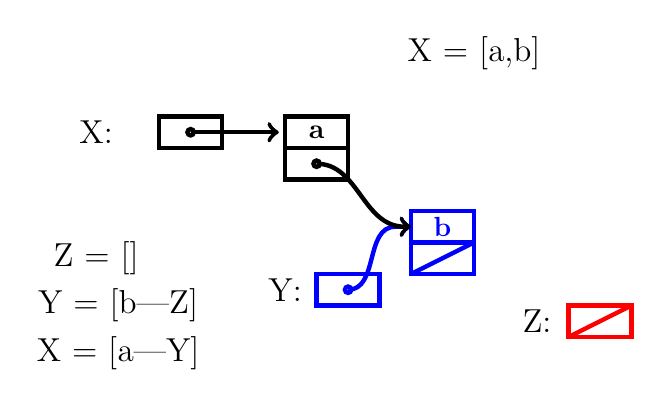
\begin{tikzpicture}[scale=0.4]


\node at (0,3.5) {{\large Z = []}};


\node at (14,1.5) {{\large Z:}};
\draw [ultra thick, red] (15,1) rectangle +(2,1);
\draw [ultra thick, red] (15,1) -- +(2,1);

\pause 
\node at (0.7,2) {{\large Y = [b|Z]}};
\pause 
\node at (6,2.5) {{\large Y:}};
\draw [ultra thick, blue] (7,2) rectangle +(2,1);
\pause 
\draw [ultra thick, blue] (10,4) rectangle +(2,1) node at +(1,0.5) {{\bf b}};
\draw [ultra thick, blue] (10,3) rectangle +(2,1);
\draw [ultra thick, blue] (10,3) -- +(2,1);
\pause 
\draw [ultra thick, blue] (8, 2.5) circle [radius =0.1];
\draw [ultra thick, blue] (8,2.5)  to [out=0, in=180]  (9.5,4.5);
\draw [ultra thick, blue, ->] (9.5,4.5) -- (10,4.5); 

\pause 
\node at (0.7,0.5) {{\large X = [a|Y]}};
\pause 
\node at (0,7.5) {{\large X:}};
\draw [ultra thick, black] (2,7) rectangle +(2,1);
\pause 
\draw [ultra thick, black] (6,7) rectangle +(2,1) node at +(1,0.5) {{\bf a}};
\draw [ultra thick, black] (6,6)  rectangle +(2,1);
\pause 

\draw [ultra thick, black] (7, 6.5) circle [radius =0.1];
\draw [ultra thick, black] (7,6.5)  to [out=0, in=180]  (9.8,4.5);
\draw [ultra thick, black, ->] (9.8, 4.5) -- (10,4.5);
\pause 
\draw [ultra thick, black] (3, 7.5) circle [radius =0.1];
\draw [ultra thick, black, ->] (3,7.5) -- (5.8, 7.5); 
\pause
\node at (12,10) {{\large X = [a,b] }};

\end{tikzpicture}

\end{frame}


\begin{frame}[fragile]{append}

\begin{verbatim}
append([], Y) -> Y;
append([H|T], Y) -> Z = append(T, Y), [ H | Z ].
\end{verbatim}

\pause
\begin{verbatim}
A = [a,b], B = [c,d], C = append(A, B).
\end{verbatim}

\pause

\begin{tikzpicture}[scale=0.4]
  
  \node at (0,8) {{\bf A:} }; 
  \cell{0.5}{8}
  \pointer{0.5}{8}{2}{6}

  \cons{2}{6}{a}
  \cdrpointer{2}{6}{6}{4}

  \cons{6}{4}{b}
  \cdrnil{6}{4}

  \node at (8,8) {{\bf B:}};
  \cell{8.5}{8}
  \pointer{8.5}{8}{12}{6}

  \cons{12}{6}{c}
  \cdrpointer{12}{6}{16}{4}

  \cons{16}{4}{d}
  \cdrnil{16}{4}


  \pause
  \cdrpointer{6}{0}{12}{6}

  \pause
  \cdrpointer{2}{0}{6}{0}
  \cons{6}{0}{b}

  \pause
  \pointer{0.5}{2}{2}{0}
  \cons{2}{0}{a}

  \pause
  \node at (0,2) {{\bf C:}};
  \cell{0.5}{2}
  \pause


\end{tikzpicture}

\end{frame}



\begin{frame}[fragile]{append}

\begin{verbatim}
append([], Y) -> Y;
append([H|T], Y) -> [ H | append(T, Y)].
\end{verbatim}

\pause\vspace{20pt} What is the {\em asymptotic time complexity} of append/2.
\end{frame}


\begin{frame}{append}

\begin{tabular}{|l|c|}
\hline
length of X & run-time in ms\\
\hline
  4000  &     50 \\
  8000  &     78 \\
 10000  &     75 \\
 12000  &     99 \\
 14000  &    102 \\
 16000  &    110 \\
 18000  &    122 \\
 20000  &    150 \\
\hline
\end{tabular}


\pause \vspace{20pt}How long time does it take to append a list of 40.000 elements?

\end{frame}

\begin{frame}{warning}

\pause The infix operator '++' is append! 

\pause\vspace{20pt} {\tt X ++ Y} is not a constant time operation!

\pause\vspace{20pt} Is {\tt [X|Y]} a constant time operation?

\end{frame}



\begin{frame}[fragile]{union of multisets}
A {\em multiset} (or bag) is a set possibly with duplicated elements.

\pause \vspace{20pt} Define a function that returns the union of two multisets.
\pause

\begin{verbatim}
union([], Y) -> Y;
union([H|T], Y) -> Z = union(T,Y), [H|Z].
\end{verbatim}

\pause \vspace{20pt} Can we do this in another way?

\pause
\begin{verbatim}
tailr([], Y) -> Y;
tailr([H|T], Y) -> Z = [H|Y], tailr(T,Z).
\end{verbatim}

\pause\vspace{20pt} Is there a difference?

\end{frame}

\begin{frame}{evaluation union}

\begin{eval}
\pause$E\lbrace\rbrace({\tt union([a,b], [c])}) \rightarrow $\\
\pause\hspace{20pt}$E\lbrace\rbrace({\tt Z = union([b], [c]), [a|Z]}) \rightarrow $\\
\pause\hspace{40pt}$E\lbrace\rbrace({\tt Z' = union([],[c]), [b|Z']}) \rightarrow $\\
\pause\hspace{60pt}$E\lbrace\rbrace({\tt [c]}) \rightarrow $\\
\pause\hspace{60pt}$[c]$\\
\pause\hspace{40pt}$E\lbrace Z'/[c]\rbrace({\tt [b|Z']}) \rightarrow $\\
\pause\hspace{40pt}$[b,c]\rightarrow $\\
\pause\hspace{20pt}$E\lbrace Z/[b,c]\rbrace({\tt [a|Z]}) \rightarrow $\\
\pause\hspace{20pt}$[a,b,c]$\\
$[a,b,c]$
\end{eval}

\end{frame}


\begin{frame}{evaluation tailr}

\begin{eval}
\pause$E\lbrace\rbrace({\tt tailr([a,b], [c])}) \rightarrow $\\
\pause\hspace{20pt}$E\lbrace\rbrace({\tt Z = [a,c], tailr([b], Z)}) \rightarrow $\\
\pause\hspace{20pt}$E\lbrace Z/[a,c]\rbrace({\tt tailr([b], Z)}) \rightarrow $\\
\pause\hspace{40pt}$E\lbrace \rbrace({\tt Z' = [b,a,c], tailr([], Z')}) \rightarrow $\\
\pause\hspace{40pt}$E\lbrace Z'/[b,a,c]\rbrace({\tt tailr([], Z')}) \rightarrow $\\
\pause\hspace{60pt}$E\lbrace \rbrace({\tt [b,a,c]}) \rightarrow $\\
\pause\hspace{60pt}$[b,a,c]$\\
\pause\hspace{40pt}$[b,a,c]$\\
\pause\hspace{20pt}$[b,a,c]$\\
$[b,a,c]$\\
\end{eval}

\end{frame}

\begin{frame}{tail recursion optimization}

When the last expression in a sequence is a function call, the stack
frame of the caller can be reused.

\pause\vspace{20pt}We call these functions {\em tail recursive}.

\pause\vspace{20pt}Possibly more efficient code.

\pause\vspace{20pt}Probably more complicated.

\pause\vspace{20pt}Very important when we will define processes!

\end{frame}

\begin{frame}[fragile]{tail recursive?}

\begin{verbatim}
sum([]) -> 0;
sum([N|T]) -> N + sum(T).
\end{verbatim}

\pause
\begin{verbatim}
sum([]) -> 0;
sum([N|T]) -> S = sum(T), N + S.
\end{verbatim}

\end{frame}

\begin{frame}[fragile]{accumulators}


\begin{verbatim}
odd([]) -> ...;
odd([H|T]) -> if H rem 2 == 1 -> ...; 
                 true -> ... 
              end.
\end{verbatim}
\pause
\begin{verbatim}
even([]) -> [];
even([H|T]) -> if H rem 2 =/= 1 -> ...; 
                  true -> ...
               end.
\end{verbatim}
\pause

\begin{verbatim}
odd_n_even(L) -> 
   Odd = odd(L),
   Even = even(L),
   {Odd, Even}.
\end{verbatim}
\end{frame}

\begin{frame}[fragile]{accumulators}

\begin{verbatim}
odd_n_even([]) ->
   {..., ...};
\end{verbatim}
\pause
\begin{verbatim}
odd_n_even([H|T]) -> 
   {Odd, Even} = odd_n_even(T),
   if 
     H rem 2 == 1 -> ...; 
     true -> ... 
   end.
\end{verbatim}

\vspace{40pt}
{\em We're building a tuple that is not needed, its only purpose is to return the two lists.}

\end{frame}


\begin{frame}[fragile]{accumulators}

\pause
\begin{verbatim}
odd_n_even(L) -> odd_n_even(L, [], []).
\end{verbatim}

\pause
\begin{verbatim}
odd_n_even([], Odd, Even) ->
   ...;
\end{verbatim}
\pause
\begin{verbatim}
odd_n_even([H|T], Odd, Even) -> 
   if 
     H rem 2 == 1 -> odd_n_even(T, ..., ...); 
     true -> odd_n_even(T, ..., ...) 
   end.
\end{verbatim}

\end{frame}

\begin{frame}[fragile]{tail recursive?}

\begin{verbatim}
sum(L) -> sum(L, ...).

sum([], S) -> ...;
sum([N|T]) -> sum(T, ...).
\end{verbatim}

\end{frame}



\begin{frame}[fragile]{flatten}

A function that {\em flattens} a list:  $${\rm flatten}([1,[2,3],4,[[5,6],[],7]]) \rightarrow [1,2,3,4,5,6,7]$$

\pause\vspace{20pt} How is this?

\pause
\begin{verbatim}
flatten([]) -> [];
\end{verbatim}
\pause\begin{verbatim}
flatten([L|T]) when is_list(L) -> flatten(L) ++ flatten(T);
\end{verbatim}
\pause\begin{verbatim}
flatten([H|T])-> [H|flatten(T)].
\end{verbatim}

\end{frame}

\begin{frame}[fragile]{flatten}


\pause\vspace{20pt} better?

\pause
\begin{verbatim}
flatten([]) -> [];
\end{verbatim}
\pause\begin{verbatim}
flatten([[]|T])-> flatten(T);
\end{verbatim}
\pause\begin{verbatim}
flatten([[H|L]|T]) -> [H | flatten([L|T])];
\end{verbatim}
\pause\begin{verbatim}
flatten([H|T]) -> [H|flatten(T)].
\end{verbatim}

\end{frame}



\begin{frame}[fragile]{naive reverse}

\pause

\begin{columns}
  \begin{column}{0.5\linewidth}
\begin{verbatim}
nrev([]) -> [];
nrev([H|T]) -> nrev(T) ++ [H].
\end{verbatim}
  \end{column}
\pause
  \begin{column}{0.5\linewidth}
\begin{verbatim}
rev(L) -> rev(L, []).

rev([], Rev) -> Rev;
rev([H|T], Rev) -> rev(T, [H|Rev]).
\end{verbatim}
  \end{column}
  \end{columns}  
\end{frame}

\begin{frame}{Summary}

\begin{itemize}
 \pause\item Pattern matching of lists - learn it by heart
 \pause\item cons - is a constant time operation
 \pause\item append - is a $O(n)$ function
 \pause\item tail recursion - a technique to master 
 \pause\item think about complexity
\end{itemize}

\end{frame}


\end{document}


